\newcommand{\labname}{Lab 2}
\documentclass[14pt]{article}
\usepackage[left=1in, right=1in, top=1in, bottom=1in]{geometry}
\usepackage{amsmath,amsfonts,amssymb}
\usepackage{graphicx}
\usepackage{fancyhdr}

% TODO: CHANGE THESE
\newcommand{\myname}{Alexander Scott Miller} % Full Name
\newcommand{\mycnetid}{amiller68} % CNetID

% header
\pagestyle{fancy}
\fancyhf{}
\lhead{CS 162 \labname}
\chead{\myname{} (\mycnetid)}
\rhead{Page \thepage{} of \pageref{mylastpagelabel}}

% document starts
\begin{document}

\paragraph{Tasks 9, 10.1, and 10.2}
\begin{figure}[htbp]
 \begin{center}
  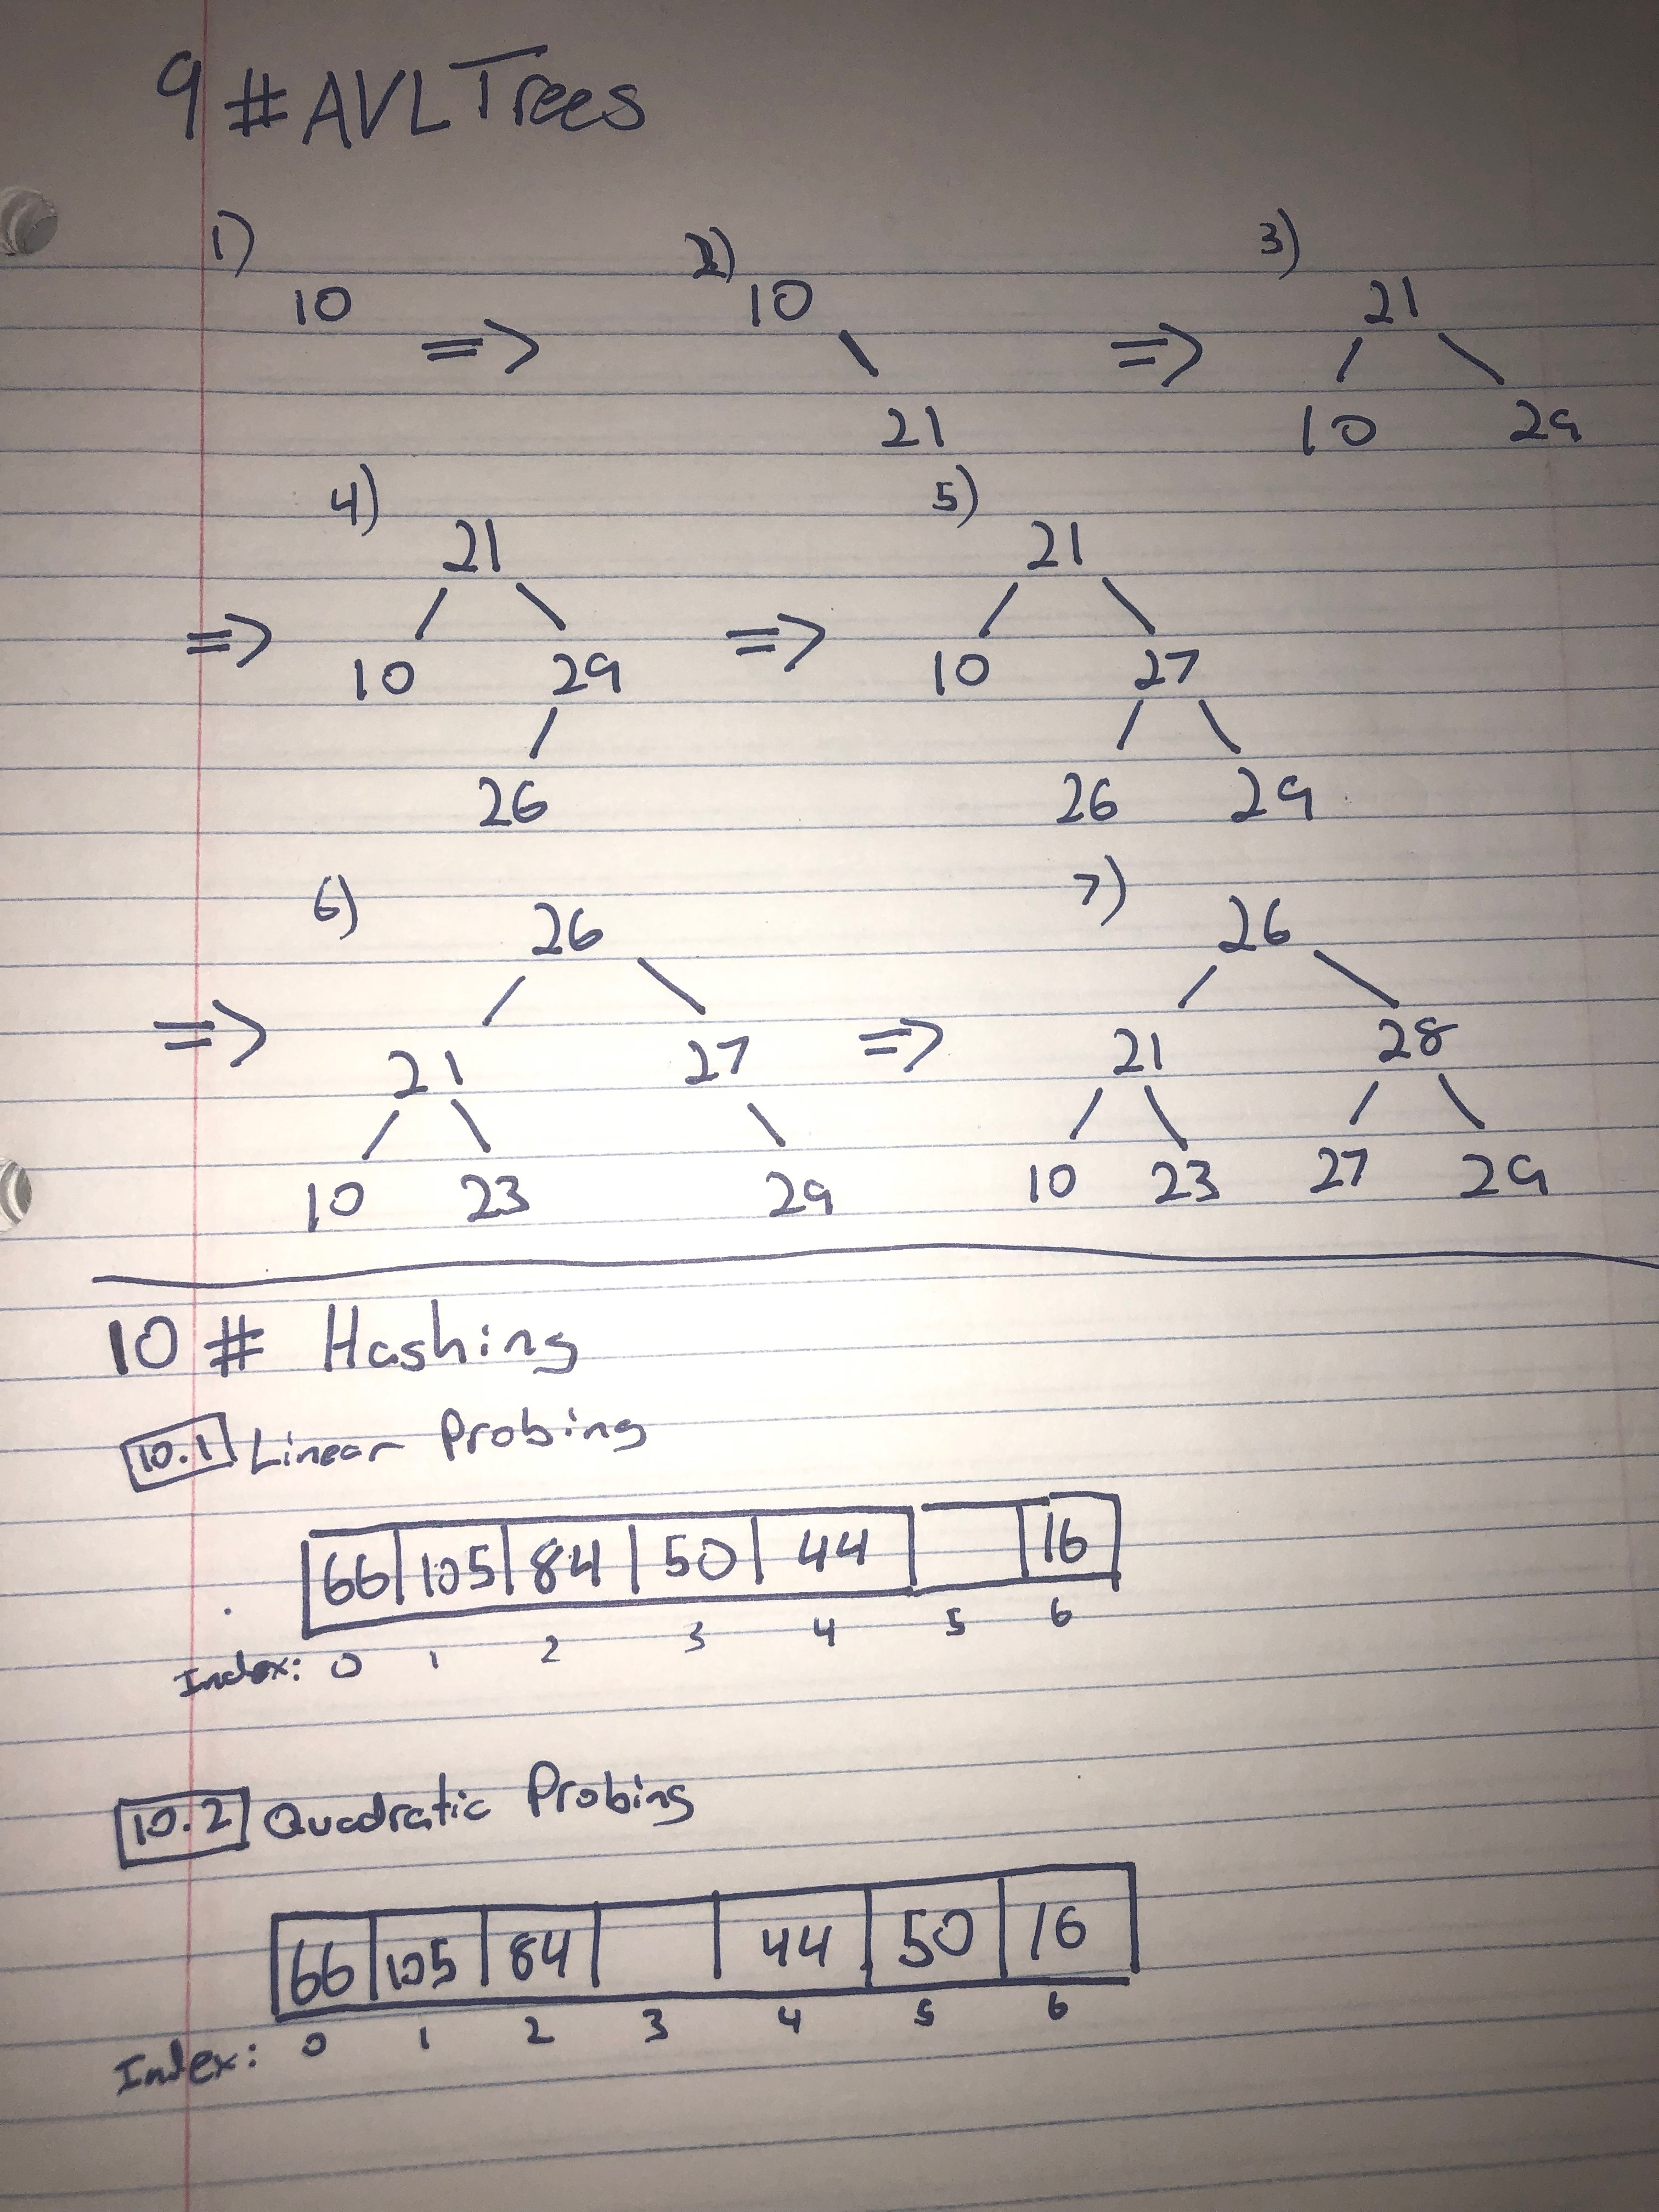
\includegraphics[width=0.5\textwidth]{pic.JPG}
  \caption{AVL Trees and hash tables}
 \end{center}
\end{figure}

\paragraph{Task 11.1}
To store 4 billion 4 byte integers in memory so that they were easily accesible would require 16 Gigabytes of RAM. This wouldn't necessarily crash my machine as it has 16 GB of RAM and any overflow could be handled by a swap partition but it would not run quickly
\paragraph{Task 11.2}
This approach would only take .5 GB of RAM. This could feasibly run on the computer I am typing this answer with as well as my phone.
\paragraph{Task 11.3}
At the start, the complexity to allocate a new ID or release an existing one is O(1). However, as the table reaches its full capacity the complexity approaches O(n). Changing the hash function won't help as it won't reduce the frequncy of collisions as the table gets closer to reaching capacity.
\paragraph{Task 11.4}
\paragraph{Task 11.5}
For keeping track of M ID numbers where M$>$0, allocate an array of unsigned chars of size (M/8) (integer division) if (M mod 8) == 0, (M/8 + 1) (integer divsion) if otherwise. Call this array Table. Make every value in this array equal 255 (integer to char conversion). Define two hash functions, hash1(x) = ((x-1) mod (M/8)) and hash(2) = ((x-1) / (M/8)). Also create an integer linked list. Call this linked list ReUse. Create a global count variable integer that is large enough to store the value of M. Call this int variable Count. Make Count = 1 to start. The process of allocate() is as follows: Check if the head of ReUse is NULL. If so check if Count$>$M. If not Table\lbrack hash1(count) \rbrack -= 2 to the power of hash2(count). Increment Count by 1. If Count>M, check if the head of ReUse is NULL. If not, take the value stored at the head of ReUSe. Call this value Hold. Table \lbrack hash1(Hold) \rbrack -= 2 to the power of hash2(Hold). Make the head of ReUse the node in the linked list following that which stored Hold. Free the node storing Hold. Keep Count the same. If Count$>$M and the head of ReUse is NULL, then there are no more IDs to allocate. The process of release(x) is as follows: Table \lbrack hash1(x) \rbrack += 2 to the power of hash2(x). Cons x to ReUse so that the head of ReUse now is a node that stores x. Return x. This implementation of the data structure makes it so that alloc() and release(x) run in O(1) time; the number of operations that either of the functions use is not dependent on the number of IDs that need to be managed. There is of course, one caveat. ReUse does take up additional memory and grows larger every time we call release(x) in succession. However, I don't think this should be a problem; in most use cases there will not be a need to remove IDs in mass and in succession without reallocating them. Therefore all processes run in O(1) time and do not require an outlandish amount of memory.    
% This label is used in the header to keep track of the page count.
\label{mylastpagelabel}

\end{document}
